\hypertarget{population_8c}{
\section{Referencia del Archivo population.c}
\label{population_8c}\index{population.c@{population.c}}
}


\subsection{Descripci\'{o}n detallada}
Definiciones del Objeto Poblacion 

Definici\'{o}n en el archivo \hyperlink{population_8c-source}{population.c}.

{\tt \#include $<$stdlib.h$>$}\par
{\tt \#include \char`\"{}population.h\char`\"{}}\par
{\tt \#include \char`\"{}genesting.h\char`\"{}}\par
{\tt \#include \char`\"{}individuo.h\char`\"{}}\par


Dependencia gr\'{a}fica adjunta para population.c:\begin{figure}[H]
\begin{center}
\leavevmode
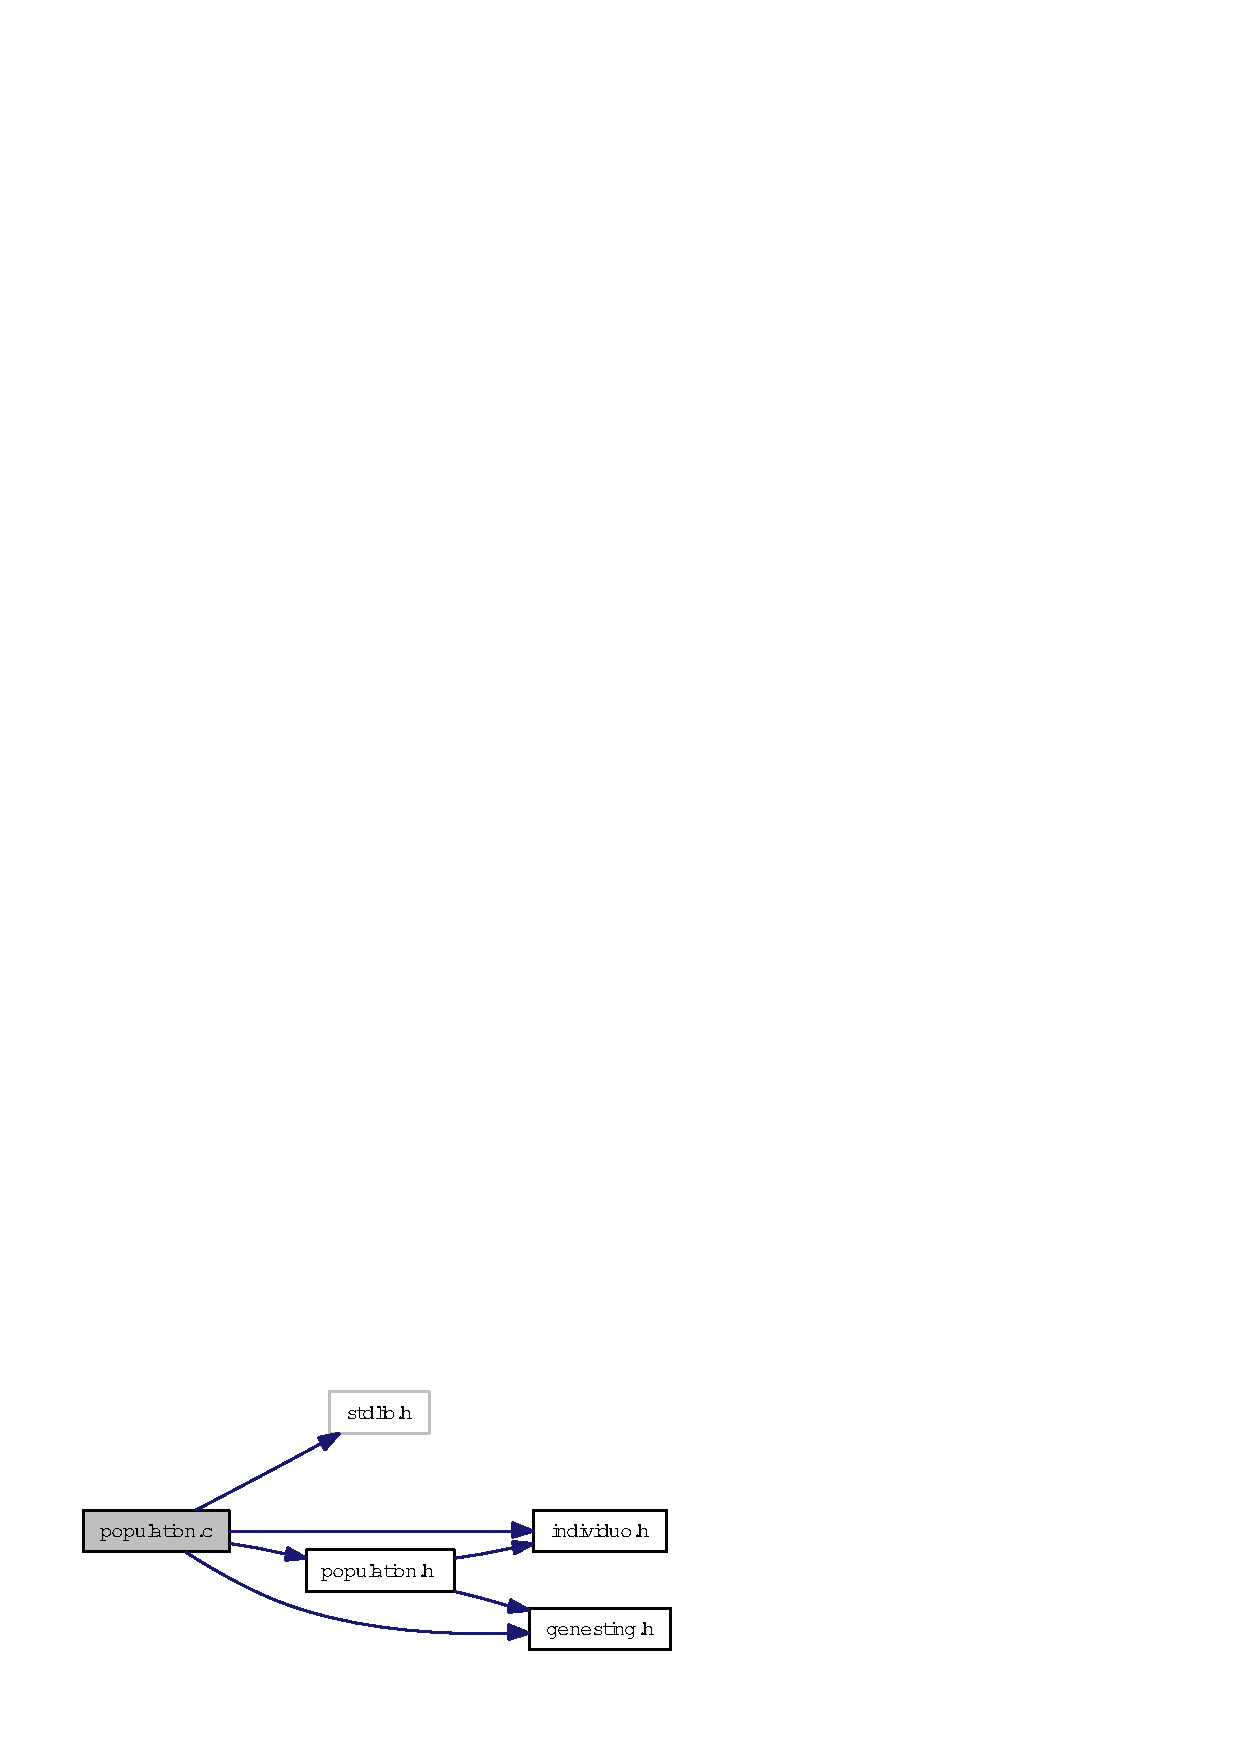
\includegraphics[width=163pt]{population_8c__incl}
\end{center}
\end{figure}
\subsection*{Funciones}
\begin{CompactItemize}
\item 
void \hyperlink{group__genetic_gc7ba874876f18abab66f0a42f32b98cc_gc7ba874876f18abab66f0a42f32b98cc}{population\_\-create} (\hyperlink{struct__population}{population} $\ast$p, \hyperlink{struct__genesting}{genesting} $\ast$g, int n)
\item 
void \hyperlink{group__genetic_g229293c432c5ef4f70b1ee94c109bb1a_g229293c432c5ef4f70b1ee94c109bb1a}{population\_\-evaluate} (\hyperlink{struct__population}{population} $\ast$p)
\item 
void \hyperlink{group__genetic_g5b3202f02e14d7fb3eb1f729d1250243_g5b3202f02e14d7fb3eb1f729d1250243}{population\_\-generation} (\hyperlink{struct__population}{population} $\ast$p)
\end{CompactItemize}
